\section{Coarse-grained Diffusion Processes}\label{chapter:RnT}
\textit{ \textbf{Acknowledgment:} the work in this section was done in close collaboration with Jacob Knight and Gunnar Pruessner}

\textit{In this section we derive a novel pertubative approach to calculating the entropy production of coarse-grained diffusion process. We then apply this technique to find the leading order contribution to the entropy production rate of an asymmetric Run-and-Tumble particle.}
\subsection{System Description}
Let $w(t)$ be any stochastic process. Consider a self-propelled particle whose motion is governed the SDE 

\begin{align}\label{main-langevin}
    \rmd x_t = \nu w(t)\rmd t +\sqrt{2D}\rmd B_t, \quad x(0) = 0,
\end{align}

where $\nu$ is a dimensionless book-keeping parameter and $B_t$ is a Brownian motion independent of $w(t)$, i.e. a Gaussian process such that
\begin{align}\label{white-noise-prop}
\begin{split}
\bE B_t &= 0 \\ 
\bE B(t)B(s) &= \min(t,s).
\end{split}
\end{align}

In the sequel, Equation (\ref{main-langevin}) and its solution will be understood in the It\^{o} sense. For the perturbation theory that follows, $w(t)$ is a generic process. Later, we will specialise to the case where $w(t)$ is an asymmetric telegraph process, such that $x(t)$ is an asymmetric Run-and-Tumble (RnT) process. An RnT process consists of intervals of constant propulsion in a fixed direction (a `run') marked by stochastic changes in the direction of propulsion (a `tumble'). In general, both the timing of tumbling events and the subsequent direction of propulsion are stochastic. In our case, $x(t)$ will be a one-dimensional RnT process where a tumbling event corresponds to a reversal in the direction of propulsion, but the timing of these events remains random. 

Here we consider the entropy production of the process $x(t)$ when $w(t)$ is hidden from the observer. Under a description that excludes the state of $w(t)$, the process $x(t)$ is no longer Markov. This is because, in general, the history of $x(t)$ contains information about the state of $w(t)$, which in turn drives the future of $x(t)$. Hence, the future, when conditioned on the present, is not independent of the past. 

This set-up is a departure from the previous sections where we have considered discrete-state, continuous-time systems. We will develop a perturbative approach for calculating the entropy production of (\ref{main-langevin}) when $w(t)$ is hidden. 

\subsection{Perturbation Theory}\label{methods}

Recall that the quantity of interest is 

\begin{align}
\entpp = \lim_{T\rightarrow \infty}\frac{1}{T}\bE \left [\log \frac{\bP[x(t)]}{\bP[x^\ast(t)]} \right],
\end{align}

where $T$ is the observation time, $\bP[x(t)]$ is the density of forward paths and $\bP[x^\ast(t)]$ is the density of reverse paths. The generator for the process $x(t)$ is 
\begin{align}
\mathcal{L} = D \frac{\rmd^2}{\rmd x^2} + \nu w(t)\frac{\rmd}{\rmd x}, 
\end{align}

so the Onsanger-Machlup function for $x(t)$ is given by \cite{capitaine1995onsager}\cite[see Chapter VI, Section 9]{ikeda1989stochastic}

\begin{align}
L(\dot{\varphi},x) = L(\dot{\varphi}) = -\frac{1}{4D}(\dot{\varphi}-\nu w(t)),
\end{align}
% The Onsanger-Machlup function for the Wiener process states that\cite{capitaine1995onsager}
hence, letting $\varphi(t)$ be any $\mathcal{C}_2$ curve such that $\varphi(0) = 0$, we have
\begin{align}
 \lim_{\epsilon \rightarrow 0} \frac{\bP\left (\norm{x - \varphi}_\infty < \epsilon  \right)}{\bP\left (\norm{x}_\infty < \epsilon  \right)} &= \exp \left (-\frac{1}{4D} \int_0^T (\dot{\varphi}(t)-\nu w(t))^2 \rmd t \right) ,
\end{align}

where $\norm{x}_\infty = \sup_{t \in [0,T]}\abs{x(t)}$ is the supremum norm on the space of continuous functions $\mathcal{C}_0([0,T], \bR)$. With some abuse of notation, we write this statement as 

\begin{align}\label{varphi-cond-prob}
\bP\left [\varphi(t)\: \lvert w(t) \right] \propto \exp \left (-\frac{1}{4D} \int_0^T (\dot{\varphi}(t) - \nu w(t))^2 \rmd t \right),
\end{align}

Equation (\ref{varphi-cond-prob}) expresses the probability that $x(t)$ will fall into a small `tube' around $\varphi(t)$ given a particular trajectory for $w(t)$. In this way, the process $x(t)$ endows the space $\mathcal{C}_2([0,T],\bR)$ with a measure which we shall denote by $\bP[\varphi(t)]$. In the interest of brevity, we introduce the notation 

\begin{align}
\begin{split}
        \Overline{F[w,\varphi]}&=\int \mathrm{D}[w(t)]\bP\left[w(t)\right]F(w,\varphi), \\
        \langle F[w,\varphi] \rangle &= \int \mathrm{D}[\varphi(t)]\bP\left [ \varphi(t) \right]F[w,\varphi],
\end{split}
\end{align}

Such that $\bE F[w,\varphi] = \left\langle \Overline{F[w,\varphi]} \right\rangle$. Here $F$ is any functional of $w$ and $\varphi$ and the notation $\mathrm{D}[\cdot]$ is used to denote a functional integral. Using this notation, we have 

\begin{align}
\begin{split}
\bP[\varphi(t)] = \Overline{\bP\left[\varphi(t)|w(t)\right]} &\propto \Overline{\exp \left\{-\frac{1}{4D} \int_0^T  \left(\dot{\varphi}-\nu w\right)^2 \rmd t \right\}}\\ 
&=  \exp \left(-\frac{1}{4D} \int_0^T  \dot{\varphi}^2 \rmd t\right) \Overline{\exp \left(-\frac{1}{4D} \int_0^T  (-2\dot{\varphi}\nu w + \nu^2 w^2) \rmd t\right)}.
\end{split}
\end{align}

Expanding the RHS of the above in small $\nu$, we discover that 

\begin{align}\label{forward-path-prob}
\small
\begin{split}
\bP[\varphi(t)] \propto &\exp \left(-\frac{1}{4D} \int \rmd t \dot{\varphi}(t)^2 \right) \bigg[1+\frac{\nu}{2D}\int \rmd t \Overline{w(t)}\dot{\varphi}(t) \\ &+ \nu^2 \left(-\frac{1}{4D}\int \rmd t \Overline{w^2(t)} + \frac{1}{8D^2}\int \rmd t_1 \rmd t_2 \Overline{w(t_1)w(t_2)}\dot{\varphi}(t_1)\dot{\varphi}(t_2)\right) \\
     &+ \nu^3 \left( -\frac{1}{8D^2}\int \rmd t_1\rmd t_2 \Overline{w^2(t_1)w(t_2)}(\dot{\varphi}(t_2) + \frac{1}{48D^3}\int \rmd t_1 \rmd t_2 \rmd t_3 \Overline{w(t_1)w(t_2)w(t_3)}\dot{\varphi}(t_1)\dot{\varphi}(t_2)\dot{\varphi}(t_3) \right) + \mathcal{O}(\nu^4) \bigg],
\end{split}
\end{align}

The time-reversed process, call it $x^\ast_t$ is governed by the same dynamics as the forward process given in Eqn (\ref{main-langevin}), however, the initial condition $x^\ast(0)$ is no longer fixed at zero, but can take on any value $x^\ast(0)= x_0 \in \bR$.\footnote{In fact the initial condition for the reverse process is not deterministic. It is given by the law of the process $x_t$ defined in (\ref{main-langevin}) at time $t = T$. But here we are concerned with the entropy production due to time-symmetry violations at the level of paths, hence we ignore the contribution due to the time-evolution of the distribution of $x_t$.} Letting $\varphi^\ast(t)$ be a $\mathcal{C}_2$ curve satisfying the initial condition $\varphi(0) = x_0$, we have 

\begin{align}
 \lim_{\epsilon \rightarrow 0} \frac{\bP\left (\norm{x^\ast - \varphi^\ast}_\infty < \epsilon  \right)}{\bP\left (\norm{x^\ast-x_0}_\infty < \epsilon  \right)} &= \exp \left (-\frac{1}{4D} \int_0^T (\dot{\varphi}(t)-\nu w(t))^2 \rmd t \right),
\end{align}
so as before
\begin{align}\label{reverse-path-prob}
\begin{split}
\bP[\varphi^\ast(t)] = \Overline{\bP\left[\varphi^\ast(t)|w(t)\right]} &\propto \Overline{\exp \left\{-\frac{1}{4D} \int_0^T  \left(\dot{\varphi}^\ast-\nu w\right)^2 \rmd t \right\}}\\ 
&=  \exp \left(-\frac{1}{4D} \int_0^T  (\dot{\varphi}^\ast)^2 \rmd t\right) \Overline{\exp \left(-\frac{1}{4D} \int_0^T  (-2\dot{\varphi}^\ast\nu w + \nu^2 w^2) \rmd t\right)},
\end{split}
\end{align}

and expanding in $\nu$ we obtain

\begin{align}\label{reverse-path-prob}
\small
\begin{split}
\bP[\varphi^\ast(t)] \propto &\exp \left(-\frac{1}{4D} \int \rmd t \dot{\varphi}^\ast(t)^2 \right) \bigg[1+\frac{\nu}{2D}\int \rmd t \Overline{w(t)}\dot{\varphi}^\ast(t) \\ &+ \nu^2 \left(-\frac{1}{4D}\int \rmd t \Overline{w^2(t)} + \frac{1}{8D^2}\int \rmd t_1 \rmd t_2 \Overline{w(t_1)w(t_2)}\dot{\varphi}^\ast(t_1)\dot{\varphi}^\ast(t_2)\right) \\
     &+ \nu^3 \left( -\frac{1}{8D^2}\int \rmd t_1\rmd t_2 \Overline{w^2(t_1)w(t_2)}(\dot{\varphi}^\ast(t_2) + \frac{1}{48D^3}\int \rmd t_1 \rmd t_2 \rmd t_3 \Overline{w(t_1)w(t_2)w(t_3)}\dot{\varphi}^\ast(t_1)\dot{\varphi}^\ast(t_2)\dot{\varphi}^\ast(t_3) \right) + \mathcal{O}(\nu^4) \bigg].
\end{split}
\end{align}

For a specific trajectory of $x_t$, we may identify $x^\ast(t) = x(T-t)$ and hence $\varphi^\ast(t) = \varphi(T-t)$. By translational symmetry, there is

\begin{align}
\frac{\bP(\norm{x}_\infty < \epsilon) }{\bP(\norm{x^\ast-x_0}_\infty < \epsilon)} = 1
\end{align}

for all $\epsilon > 0$, hence the constants of proportionality in Eqns. (\ref{forward-path-prob}) and (\ref{reverse-path-prob}) are equal. Hence we can write 

\begin{align}\label{reverse-path-prob-expanded}
\small
\begin{split}
\bP[\varphi^\ast(t)] = \bP[\varphi(T-t)] \propto &\exp \left(-\frac{1}{4D} \int \rmd s \dot{\varphi}(s)^2 \right) \bigg[1-\frac{\nu}{2D}\int \rmd s \Overline{w(s)}\dot{\varphi}(s) \\ &+ \nu^2 \left(-\frac{1}{4D}\int \rmd s \Overline{w^2(s)} + \frac{1}{8D^2}\int \rmd s_1 \rmd s_2 \Overline{w(s_1)w(s_2)}\dot{\varphi}(s_1)\dot{\varphi}(s_2)\right) \\
     &+ \nu^3 \bigg( \frac{1}{8D^2}\int \rmd s_1\rmd s_2 \Overline{w^2(s_1)w(s_2)}\dot{\varphi}(s_2) \\&- \frac{1}{48D^3}\int \rmd s_1 \rmd s_2 \rmd s_3 \Overline{w(s_1)w(s_2)w(s_3)}\dot{\varphi}(s_1)\dot{\varphi}(s_2)\dot{\varphi}(s_3)\bigg) + \mathcal{O}(\nu^4) \bigg],
\end{split}
\end{align}

where we have made use of the change of variable $s = T-t$. Observe that in the expansion for the reverse path probability in (\ref{reverse-path-prob-expanded}), terms that are odd in $\dot{\varphi}$ have opposite signs to their counterpart in the expansion (\ref{forward-path-prob}). On the other hand, terms that are even in $\dot{\varphi}$ have the same sign in both expressions. Since the constants of proportionality in (\ref{forward-path-prob}) and (\ref{reverse-path-prob}) are equal, we have the path-wise entropy production rate functional

\begin{align}
\dot{S}[\varphi]  \coloneqq \frac{1}{T}\log \frac{\bP[\varphi]}{\bP[\varphi^\ast]} = \frac{1}{T}\log \frac{\bP[\varphi(t)]}{\bP[\varphi(T-t)]}.
\end{align}

Upon expanding $S[\varphi]$ in $\nu$ and taking note of cancellations one obtains 

\begin{equation}\small\label{onepath}
\begin{split}
 \dot{S}[\varphi(t)] = & \frac{1}{T}\log\left(\frac{\bP\left[\dot{\varphi}(t)\right]}{\bP\left[\dot{\varphi}(t)^\ast\right]}\right) \\= & \frac{\nu}{TD}\int_0^T\rmd t\dot{\varphi}(t)\Overline{w(t)} \\
 &+ \frac{\nu^3}{T} \bigg[\frac{1}{4D^2} \int_0^T \rmd t_1 \rmd t_2 \Overline{w(t_1)}\cdot\Overline{w(t_2)^2}\dot{\varphi}(t_1) + \frac{1}{24D^3}\int_0^T \rmd t_1 \rmd t_2 \rmd t_3 \Overline{w(t_1)w(t_2)w(t_3)}\dot{\varphi}(t_1)\dot{\varphi}(t_2)\dot{\varphi}(t_3)\\
  &- \frac{1}{8D^3}\int_0^T \rmd t_1 \rmd t_2 \rmd t_3 \Overline{w(t_1)}\cdot \Overline{w(t_2)w(t_3)}\dot{\varphi}(t_1)\dot{\varphi}(t_2)\dot{\varphi}(t_3)\bigg] + \mathcal{O}(\nu^4)
\end{split}
\end{equation}

We now make the following claim without proof. \\

\textit{\textbf{Claim:}
The autocorrelators of $\dot{\varphi}$ are equal to the autocorrelatros of $\nu w$ except possibly on the diagonal set $\{(t_1,\ldots,t_n): t_1 = t_2 \ldots = t_n\}$, i.e.,}

\begin{align}
\langle \dot{\varphi}(t_1)\ldots\dot{\varphi}(t_n)\rangle = \nu^n\Overline{w(t_1)\ldots w(t_n)} + K(t_1)\mathds{1}_{\{t_1 =t_2 \ldots =t_n\}}.
\end{align}

\textit{where $K$ is an unknown function and $\mathds{1}_A$ is the indicator function of $A$.}

As a consequence of the Stone-Weierstrass theorem $x(t)$ can be approximated arbitrarily well by $\mathcal{C}_2$ functions (in the sense of $\norm{\cdot}_\infty$). Hence, $\dot{\varphi}(t)$ can be viewed as a smooth approximation of the increments of $x(t)$.\footenote{A most crucial question here is ``In what sense does $\dot{\varphi(t)}$ approximate the increments of $x(t)$?'' Answering this question would make rigorous the intuition we have outlined in support of the claim.} The increments of $x(t)$ are composed of contribution of the form $\nu w(t)\delta t$ plus Brownian increments. Brownian increments from disjoint time segments are independent. Hence the claim. Assuming the claim, the expected entropy production rate is

\begin{align}\label{expected-entropy-gen}
\begin{split}
\entpp &= \lim_{T\rightarrow \infty}\langle \dot{S}[\varphi] \rangle \\ 
&= \frac{\nu^2}{TD}\int_0^T\rmd t\left(\Overline{w(t)}\right)^2 \\
 &+ \frac{\nu^4}{4TD^2} \int_0^T \rmd t_1 \rmd t_2 \Overline{w(t_2)^2}\cdot\left(\Overline{w(t_1)}\right)^2\\ 
 &+ \frac{\nu^6}{T}\bigg[\frac{1}{24D^3}\int_0^T \rmd t_1 \rmd t_2 \rmd t_3 \left(\Overline{w(t_1)w(t_2)w(t_3)}\right)^2\\
  &- \frac{1}{8D^3}\int_0^T \Overline{w(t_1)}\cdot \Overline{w(t_2)w(t_3)}\cdot\Overline{w(t_1)w(t_2)w(t_3)}\bigg] + \mathcal{O}(\nu^8)
\end{split}
\end{align}

In obtaining this expression for $\entpp$ we have ignored terms of the form $K(t_1)\mathds{1}_{\{t_1 = t_2 \ldots = t_n\}}$ since the set $\{t_1 = t_2 \ldots = t_n\}$ has zero measure. If the process $w(t)$ has zero mean (i.e. zero current), $\Overline{w(t)} = 0$, then Eqn. (\ref{expected-entropy-gen}) reduces to 

\begin{align}\label{zero-mean-entropy}
\entpp = \frac{\nu^6}{24TD^3}\int_0^T \rmd t_1 \rmd t_2 \rmd t_3 \left(\Overline{w(t_1)w(t_2)w(t_3)}\right)^2 + \mathcal{O}(\nu^8)
\end{align}


\subsection{Asymmetric RnT Process}\label{subsection:asymmetric-RnT}

We now specialise to the case where $w(t)$ is a mean-zero asymmetric telegraph process. The telegraph process $w(t) \in \{w_+, w_-\}$ evolves according to 

\begin{align}
\begin{split}
\bP(w(t+\delta t) = w_+ | w(t) = w_-) &= \alpha_- \delta t \\ 
\bP(w(t+\delta t) = w_- | w(t) = w_+) &= \alpha_+ \delta t.
\end{split}
\end{align}

for $\alpha_+, \alpha_- \geq 0$ and for small time $\delta t$, and the mean-zero condition 

\begin{align}\label{zero-mean}
    \Overline{w(t)} = \frac{w_+\alpha_- + w_-\alpha_+}{\alpha_+ + \alpha_-} = 0,
\end{align}

is satisfied. 

\begin{figure}
\centering
\subfloat[Asymmetric telegraph process.\label{telegraph_diagram}]{%
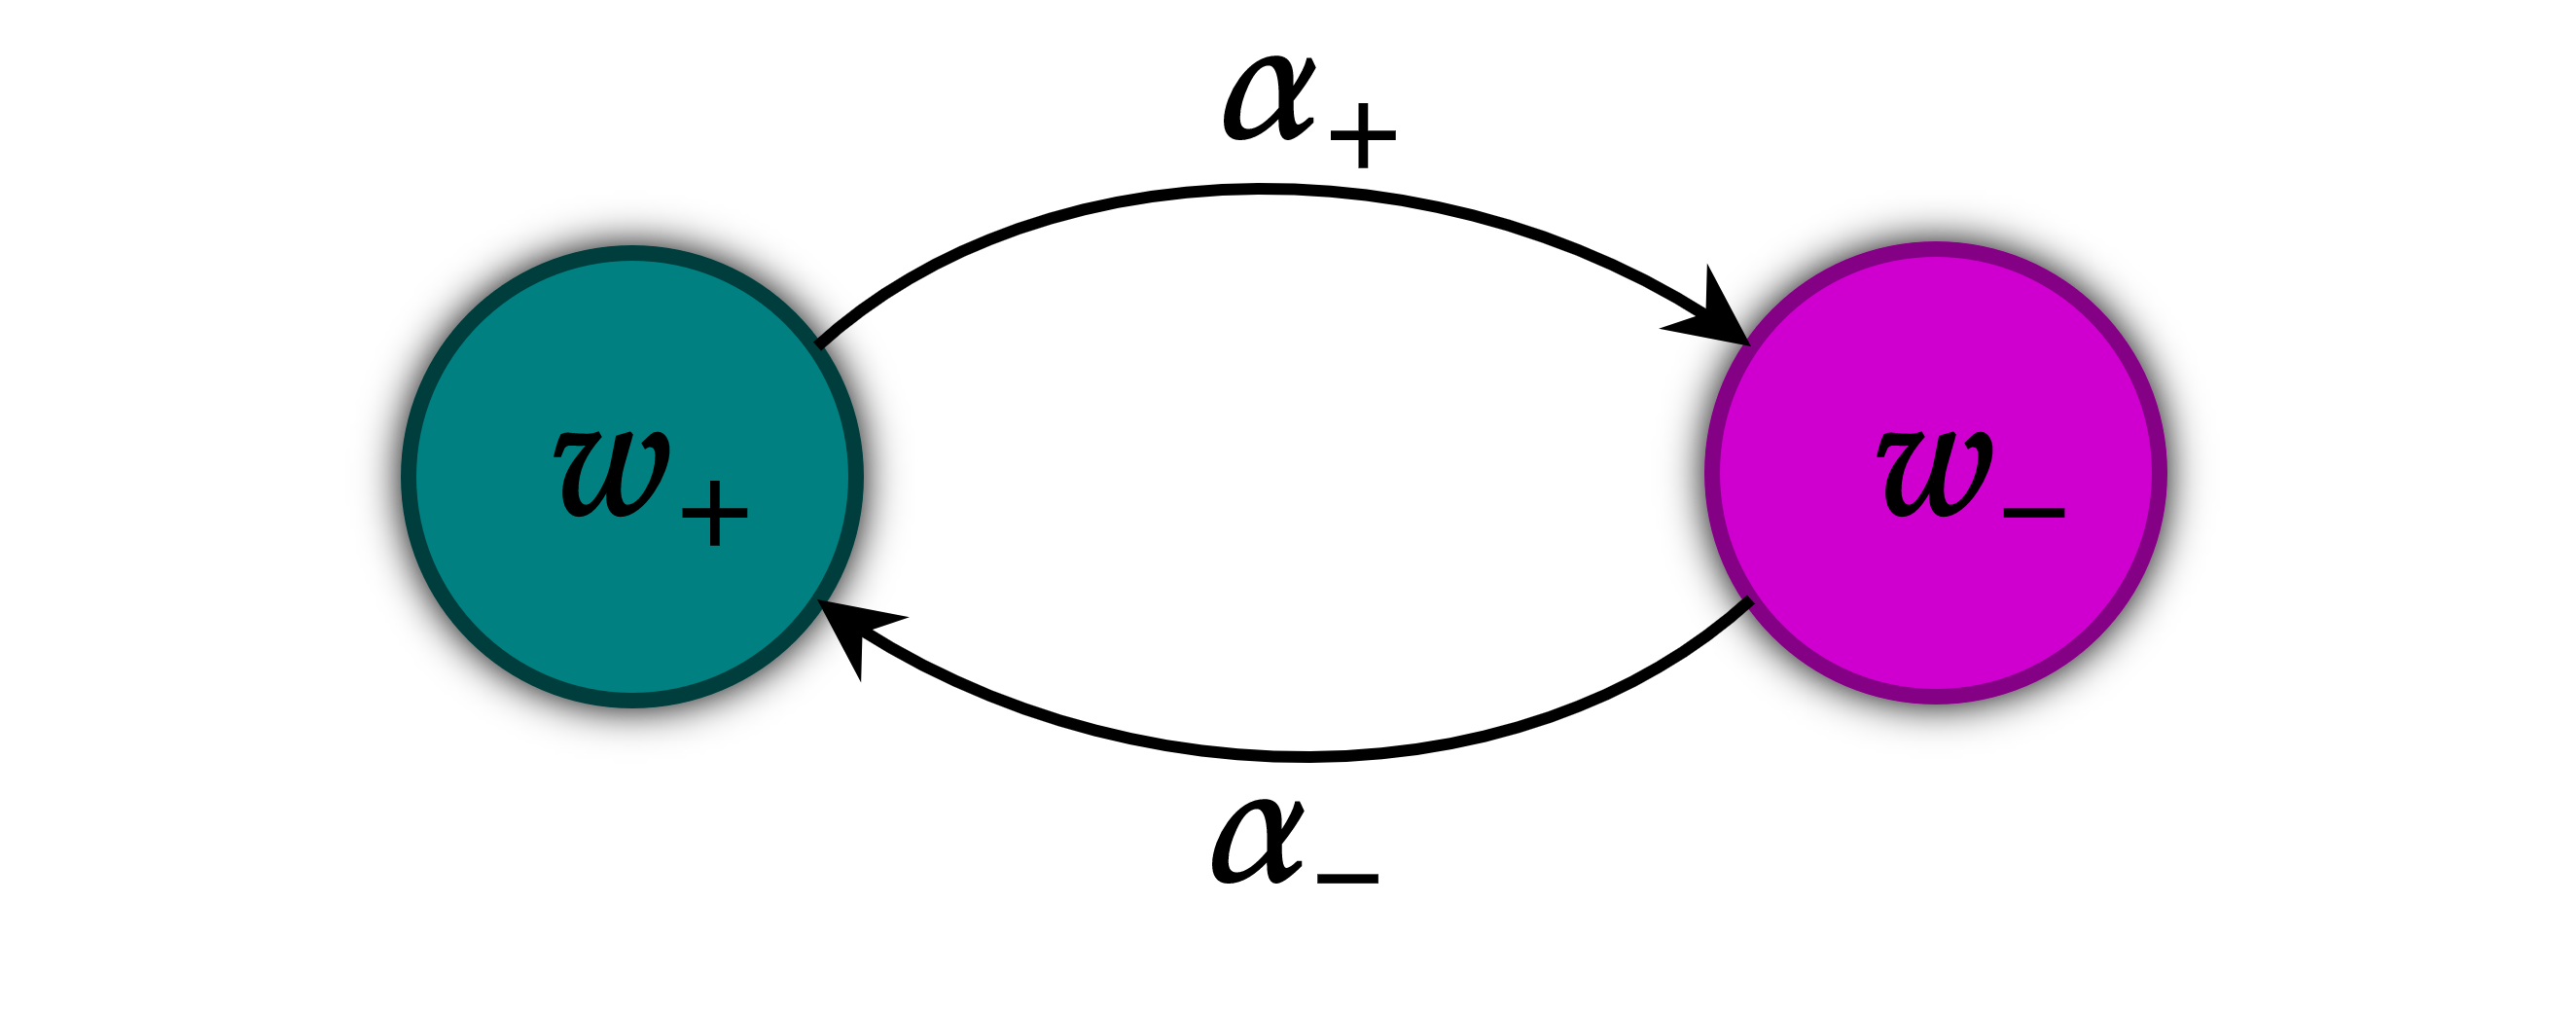
\includegraphics[width = 0.49\textwidth]{figures/tele-diagram-w3.png}}
\hfill
\subfloat[A Sample path for the asymmetric RnT particle.\label{sample_path}]{%
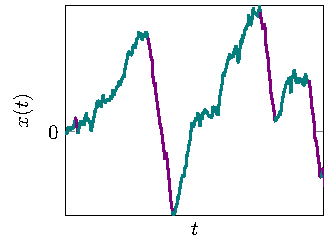
\includegraphics[width = 0.49\textwidth]{figures/RnT_sample_path.pdf}
}
\caption{\footnotesize Subfigure \ref{telegraph_diagram} shows a diagram of the telegraph process $w(t)$ as discussed in Subsection \ref{subsection:asymmetric-RnT}. In the +ve state, the particle has self-propulsion $\nu w_+$, and in the -ve state the self-propulsion is $\nu w_-$. Since $\Overline{w} = 0$, we have $\alpha_+w_- + \alpha_-w_+ = 0$. Subfigure \ref{sample_path} depicts a sample path for the particle governed by (\ref{main-langevin}) where $w(t)$ is an asymmetric telegraph process with zero mean. The green and purple line segments indicates the state of the driving telegraph process, corresponding to velocities $w_+$ and $w_-$ respectively. For this sample path we have set $\abs{w_-/w_+}= 5$.}
\label{figure1}
\end{figure}

According to Eqn. (\ref{zero-mean-entropy}), the leading order contribution to the entropy production rate of $x_t$ is 

\begin{align}\label{RnT-entroppy-int}
\entpp = \frac{\nu^6}{24TD^3}\int_0^T \rmd t_1 \rmd t_2 \rmd t_3 \left(\Overline{w(t_1)w(t_2)w(t_3)}\right)^2. 
\end{align}

In order to calculate the three-time correlation $\Overline{w(t_1)w(t_2)w(t_3)}$, begin from the master equation for the evolution of $w(t)$, 

\begin{equation}
\frac{\rmd}{\rmd t}\begin{pmatrix}
p_+(t) \\
p_-(t)
\end{pmatrix} =
\begin{pmatrix}
-\alpha_+ & \alpha_- \\
\alpha_+  & -\alpha_-
\end{pmatrix}
\begin{pmatrix}
p_+(t) \\
p_-(t)
\end{pmatrix}.
\end{equation}

Here $p_+(t)$ is the probability of the event $w(t) = w_+$ and $p_-(t)$ is the probability of the event $w(t) = w_-$. Solving this system with appropriate boundary conditions, one obtains the propagators  

\begin{equation}\label{elements}
    \begin{split}
        P_{++}(t) &= \frac{1}{\alpha_+ + \alpha_-} \left(\alpha_- + \alpha_+ e^{-(\alpha_+ + \alpha_-)t}\right) \\
        P_{-+}(t) &= \frac{1}{\alpha_+ + \alpha_-} \left(\alpha_+ - \alpha_+ e^{-(\alpha_+ + \alpha_-)t}\right) \\
        P_{+-}(t) &= \frac{1}{\alpha_+ + \alpha_-} \left(\alpha_- - \alpha_- e^{-(\alpha_+ + \alpha_-)t}\right) \\
        P_{--}(t) &= \frac{1}{\alpha_+ + \alpha_-} \left(\alpha_+ + \alpha_- e^{-(\alpha_+ + \alpha_-)t}\right) \\
    \end{split}
\end{equation}
where $P_{ij}(t)$ is the probability of $w(t)$ taking a value $w_i$ having been initialised at $t=0$ with value $w_j$, for $i,j \in \{+ , -\}$. The three-time correlation function of $w(t)$ is then 

\begin{equation}\label{3time}
\begin{split}
    \Overline{w(t_3)w(t_2)w(t_1)} =& \mathds{1}_{\{t_3>t_2>t_1\}}
 \begin{pmatrix}
1 & 1\\
\end{pmatrix}
M_{w}(t_3-t_{2})M_{w}(t_2-t_{1})
\begin{pmatrix}
w_+P_{+}\\
w_-P_{-}
\end{pmatrix}\\
&+\mathds{1}_{\{t_2>t_3>t_1\}}
 \begin{pmatrix}
1 & 1\\
\end{pmatrix}
M_{w}(t_2-t_{3})M_{w}(t_3-t_{1})
\begin{pmatrix}
w_+P_{+}\\
w_-P_{-}
\end{pmatrix} + \cdots
\end{split}
\end{equation}

where $P_{+/-}=\lim_{t \to \infty} P_{++/--}(t)$ are the stationary probabilities of $w(t)$ taking the value $w_{+/-}$ and $\mathds{1}_{\{t_3>t_2>t_1\}}$ are indicator functions which impose time-ordering. The transition matrix $M_w(t)$ is given by 

\begin{align}
    M_{w}(t) &= \begin{pmatrix}
w_+P_{++}(t) & w_+P_{+-}(t) \\
w_-P_{-+}(t)  & w_-P_{--}(t)
\end{pmatrix} \\ 
&= M_{w0} + M_{w1}e^{-(\alpha_+ + \alpha_-)t},
\end{align}

where 
\begin{align}
\begin{split}
M_{w0} &= \frac{1}{\alpha_+ + \alpha_-} \begin{pmatrix}
        w_+\alpha_- & w_+\alpha_- \\
        w_-\alpha_+ & w_-\alpha_+
        \end{pmatrix} \\
        M_{w1} &= \frac{1}{\alpha_+ + \alpha_-} \begin{pmatrix}
        w_+\alpha_+ & -w_+\alpha_- \\
        -w_-\alpha_+ & w_-\alpha_-
        \end{pmatrix}.
\end{split}
\end{align}

Eqn. (\ref{3time}) can be simplified using the relation 

\begin{equation}\label{3time2}
     \begin{pmatrix}
1 & 1\\
\end{pmatrix}M_{w0} = M_{w0}
\begin{pmatrix}
w_+P_{+}\\
w_-P_{-}
\end{pmatrix} = 0.
\end{equation}

The three-time correlation $\Overline{w(t_1)w(t_2)w(t_3)}$ is then given by 

\begin{equation}
\begin{split}
        \Overline{w(t_3)w(t_2)w(t_1)} &= \mathds{1}_{\{t_3>t_2>t_1\}}
 \begin{pmatrix}
1 & 1\\
\end{pmatrix}
M_{w1}^2
\begin{pmatrix}
w_+P_{+}\\
w_-P_{-}
\end{pmatrix} e^{-(\alpha_+ + \alpha_-)(t_3-t_1)} +  \\ &\quad \quad \mathds{1}_{\{t_2>t_3>t_1\}}
 \begin{pmatrix}
1 & 1\\
\end{pmatrix}
M_{w1}^2
\begin{pmatrix}
w_+P_{+}\\
w_-P_{-}
\end{pmatrix} e^{-(\alpha_+ + \alpha_-)(t_2-t_1)}\\
&= \frac{\alpha_+ \alpha_- (\alpha_+ w_+ + \alpha_- w_-)(w_+ - w_-)^2}{(\alpha_+ + \alpha_-)^3}\times \\ &\quad \quad \Big[ e^{-(\alpha_+ + \alpha_-)(t_3-t_1)}\mathds{1}_{\{t_3>t_2>t_1\}} + e^{-(\alpha_+ + \alpha_-)(t_2-t_1)}\mathds{1}_{\{t_2>t_3>t_1\}} + \cdots \Big]
\end{split}
\end{equation}

Using this expression in Eqn. (\ref{RnT-entroppy-int}), we obtain

\begin{align}
    \begin{split}
     \dot{\mathcal{S}}=  \frac{\nu^6}{4\cdot3!\cdot T D^3}\Bigg[\frac{\alpha_+ \alpha_- (\alpha_+ w_+ + \alpha_- w_-)(w_+ - w_-)^2}{(\alpha_+ + \alpha_-)^3}\Bigg]^2 \int_0^T\rmd t_1\rmd t_2\rmd t_3\Big[ & e^{-(\alpha_+ + \alpha_-)(t_3-t_1)}\mathds{1}_{\{(t_3>t_2>t_1\}} \\&+ e^{-(\alpha_+ + \alpha_-)(t_2-t_1)}\mathds{1}{\{t_2>t_3>t_1\}} + \cdots \Big]^2,
\end{split}
\end{align}

which evaluates to
\begin{align}
    \begin{split}
 \dot{\mathcal{S}}&=  \frac{\nu^6}{4\cdot3!\cdot T D^3}\Bigg[\frac{\alpha_+ \alpha_- (\alpha_+ w_+ + \alpha_- w_-)(w_+ - w_-)^2}{(\alpha_+ + \alpha_-)^3}\Bigg]^2\cdot 6 \int_0^T\rmd t_3\int_0^{t_3}\rmd t_2\int_0^{t_2}\rmd t_1  e^{-2(\alpha_+ + \alpha_-)(t_3-t_1)}\\
 &=\frac{\nu^6}{16 T D^3}\cdot \frac{\alpha_+^2 \alpha_-^2 (\alpha_+ w_+ + \alpha_- w_-)^2(w_+ - w_-)^4}{(\alpha_+ + \alpha_-)^8}
\end{split}
\end{align}

Finally, we use the zero-mean condition (\ref{zero-mean}) to obtain 

\begin{align}\label{RnT-ent}
\dot{\mathcal{S}}=-\frac{\nu^6}{16D^3}\cdot\frac{w_+^3w_-^3}{\alpha_+\alpha_-}\left(\frac{\alpha_+-\alpha_-}{\alpha_+ + \alpha_-}\right)^2
\end{align}

We may furthermore define the geometric average transitions rate $\bar{\alpha}= \sqrt{\alpha_+\alpha_-}$ and the geometric average speed $\bar{\omega} = \sqrt{\abs{w_+w_-}}$ to arrive at 

\begin{align}
  \dot{\mathcal{S}} = \frac{\nu^6}{16D^3}\frac{\bar{w}^6}{\bar{\alpha}^2}\left(\frac{1-\lambda}{1+\lambda}\right)^2,
\end{align}

where 

\begin{equation}
  \lambda \coloneqq \abs{\frac{w_-}{w_+}} = \frac{\alpha_-}{\alpha_+}.
\end{equation}

\subsection{Discussion}
\subsubsection{Entropy Production Results}

In Subsection \ref{methods} we present a perturbative framework for calculating the entropy production of self-propelling particles subject to a potential. In general, obtaining a closed form expression may be difficult when using this framework. However, in particular cases of interest, such as when the net current is zero, the calculations simplify considerably, allowing us to obtain closed-form expressions for the leading order contributions to entropy production.

In Subsection \ref{subsection:asymmetric-RnT} we derive the leading order contribution to the entropy production for a free asymmetric RnT particle. This is given by

\begin{equation}\label{RnT-ent-geom}
  \dot{\mathcal{S}} = \frac{\nu^6}{16D^3}\frac{\bar{w}^6}{\bar{\alpha}^2}\left(\frac{1-\lambda}{1+\lambda}\right)^2,
\end{equation}

where $\bar{w} = \sqrt{\abs{w_+w_-}}$ and $\bar{\alpha} = \sqrt{\alpha_+\alpha_-}$ are the geometric average speed and transition rate respectively, and

\begin{equation}
  \lambda \coloneqq \abs{\frac{w_-}{w_+}} = \frac{\alpha_-}{\alpha_+}.
\end{equation}

Eqn. (\ref{RnT-ent-geom}) illuminates the dependence of $\dot{\mathcal{S}}$ on the ratio of the speeds, $\lambda$. The entropy production disappears at $\lambda = 1$ as expected. For fixed values of $\bar{w}$ and $\bar{\alpha}$ the maximum entropy production

\begin{equation}\label{max_entropy}
  \dot{\mathcal{S}}_{\text{max}} = \frac{\nu^6}{16D^3}\frac{\bar{w}^6}{\bar{\alpha}^2}
\end{equation}

is achieved in the limit as $\lambda \rightarrow \infty$. This is consistent with the `Unexpected state mechanism' which we subsequently propose in Subsection \ref{EPmechanism}. The limit as $\lambda \rightarrow 0$ requires careful treatment. If this limit is taken by keeping $w_+, \alpha_+$ fixed and sending $w_-,\alpha_- \rightarrow 0$, then the resulting process will have zero entropy production. If, on the other hand the limit $\lambda \rightarrow 0$ is taken by fixing $w_-$ and sending $w_+ \rightarrow \infty$, the resulting process tends towards infinite entropy production. When $\lambda = 0$, we have that in the stationary state 
$\mathcal{P}\left[w(t) = w_-\right] = 1$, and hence as $w(t)$ approaches its equilibrium state, $x(t)$ behaves as an unforced Brownian motion with zero entropy production.

In the strong diffusion regime where $D \gg \bar{w}^2/\bar{\alpha}$, the noise dominates the self-propulsion kinetics and the entropy production disappears. In other words, the entropy production becomes negligible whenever $\bar{\alpha} \gg \bar{w}^2/D$. The factor $\bar{w}^2/D$ is analogues to the $v^2/D$ term which appears in the entropy production of a diffusion process with constant self-propulsion speed $v$\cite{cocconi2020entropy}. When the condition $\bar{\alpha} \gg \bar{w}^2/D$ is satisfied, the high transition rate effectively masks the self-propulsion of the particle, resulting in reduced entropy production.

\subsubsection{Entropy Production Mechanism}\label{EPmechanism}

\begin{wrapfigure}{R}{0.5\textwidth}
    \centering
    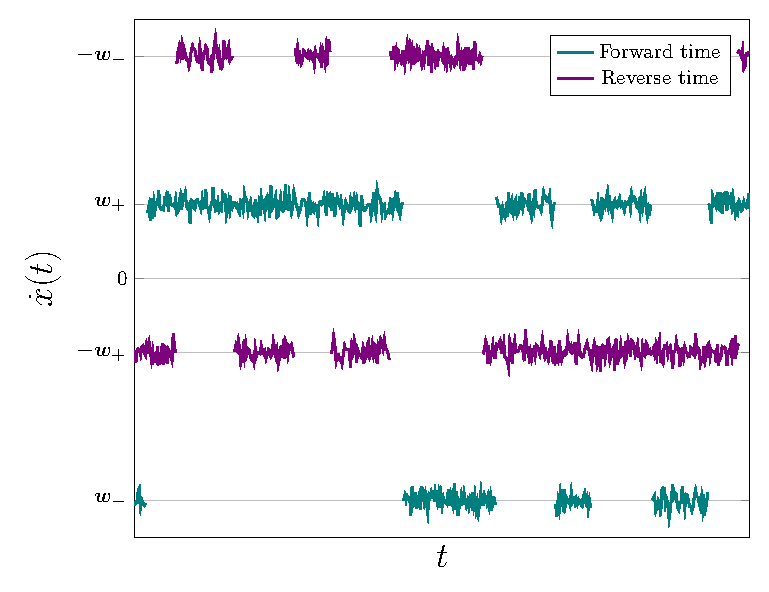
\includegraphics[width = 0.45\textwidth]{figures/unexpected_state.pdf}
    \caption{\footnotesize The observed velocities for a sample path of the asymmetric RnT process when time is run forwards (green/blue) and backwards (purple). Entropy production arises because time reversal results in the `unexpected' states $-w_-$ and $-w_+$ for the velocity. Maintaining these states has a high probability cost in terms of the noise, hence the different statistics of forward and reverse paths. Note that the forward path is simply the sum of a telegraph process and white noise, so it is time reversible. It is precisely the appearance of unexpected velocity states under time reversal that results in entropy production.} 
   \label{unexpeced_states}
\end{wrapfigure}

We have shown that the process $x(t)$ defined by (\ref{main-langevin}) has non-zero entropy production in its steady-state, even when $w(t)$ is hidden from the observer. However, the underlying telegraph process, $w(t)$, and white noise, $\xi(t)$, \textit{are} time reversible. Explicitly, the process defined by

\begin{equation}
\dot{y}(t) = \nu w(T-t) + \xi(T-t), \quad y(0) = 0, t \in [0, T]
\end{equation}

 has identical statistics to the process defined by (\ref{main-langevin}).  This provokes the following question: how can time-reversible underlying processes give rise to trajectories which are \textit{distinguishable} from their time-reverse? 
 The answer lies in the physical variables to which the processes are coupled. In equation (\ref{main-langevin}), the telegraph process represents a velocity. When time is reversed, not only is the trajectory of the telegraph process reversed, but also the sign of the velocity associated with that state. The result is the appearance of the `unexpected' states $-w_-$ and $-w_+$ in the velocity profile of the particle (figure \ref{unexpeced_states}). These unexpected states can only be maintained through persistent noise against the self-propulsion direction, which incurs a high probability cost according to Eqn. (\ref{varphi-cond-prob}). Put another way, the entropy production of the asymmetric RnT process results from the identity\footnote{This identity is only formal, since $x(t)$ is a.s. not differentiable. It can be interpreted as a statement about the increments of $x(t)$.}

\begin{equation}
\frac{\rmd x}{\rmd s}(s) = -\dot{x}(t),
\end{equation}

where $s = T-t$ is the reverse-time variable. But $-\dot{x}(t)$ does not result from the time reversal of the underlying mechanisms, i.e., the processes $x(s)$ and $y(t)$ are not equal in law. This observation emphasises the need to distinguish between the effect of time-reversal on the time-dependent parts of the dynamics (e.g. telegraphic noise) and the nature of the states themselves, which change in a time-independent way.



